\documentclass[12pt]{article}
\usepackage{geometry}
\usepackage{amsmath, amssymb}
\usepackage[amssymb]{SIunits}
\usepackage{tikz, pgfplots}
\usepackage{xcolor-material}
\usepackage[htt]{hyphenat}
\usepackage{caption}
\usepackage{subcaption}
\usepackage{biblatex}
\addbibresource{ref.bib}

\usepackage{sectsty}
\sectionfont{\color{MaterialBlueGrey800} \MakeUppercase} 
\subsectionfont{\color{MaterialBlueGrey700} \MakeUppercase}
\subsubsectionfont{\color{MaterialBlueGrey600} \MakeUppercase}

% Code settings
\usepackage{listings}
\lstset{basicstyle=\ttfamily}

\usepackage{hyperref}
\hypersetup{
	colorlinks=true,
	linkcolor=MaterialBlue
	filecolor=MaterialBlue,
	urlcolor=MaterialBlue,
}

% Geometry setup
\geometry{
	a4paper,
	hscale=0.618, 
	vscale=0.85,
	hcentering,
	marginparsep=5mm,
	marginparwidth=16ex,
}

% Use these modification for basic commands settings
\renewcommand{\vec}{\boldsymbol}

% Set indent
\setlength{\parindent}{0em}
\setlength{\parskip}{1.5ex}

\makeatletter
\def\@maketitle{%
	\newpage
	\null
	\noindent\rule{\textwidth}{0.4pt}
	\begin{center}
		{\Large \scshape \@title \par}
		{%
			\large
			\begin{tabular}[t]{c}
				{\scshape \@author}
			\end{tabular}
		}\par
	\noindent\rule{\textwidth}{0.4pt}
	\end{center}
	\vskip 1.5em}
\makeatother

\usepackage[english]{babel}
\usepackage{blindtext}
\usepackage[framemethod=TikZ]{mdframed}
\mdfsetup{%
	topline=false,
	bottomline=false,
	skipabove=\topsep,
	skipbelow=\topsep,
	linecolor=MaterialBlueGrey500
}
\surroundwithmdframed{quote}

% margin par settings
\let \oldmarginpar \marginpar
\renewcommand{\marginpar}[1]{%
	\oldmarginpar{%
		\begin{mdframed}[%
			rightline=false,
			innerleftmargin=4pt,
			linewidth=1pt,
		]
			\tiny \color{MaterialBlueGrey500} \sffamily
			\setlength{\baselineskip}{1.25em}
			#1
		\end{mdframed}
}}

% 
% !!! User-specified options !!!
%
\title{Parallel Breadth-First Search on Multi-Core CPU in OpenMP}
\author{Zike (Kevin) XU \quad 2020533081}
\date{\today}

\begin{document}

\maketitle

\section{Introduction}
 {\scshape BFS} in modern computer science can be used in many cases. For example, benchmarking super-computers with BFS can effectively test some crucial aspects that common benchmarking utils cannot touch. Analyzing anything that can be represented as a graph requires traversing algorithms like BFS. These graphs can be large, which imposed a daunting challenge on the graph-processing program.


In this lab, we'll implement the three common types of BFS: \textit{\color{MaterialBlueGrey} Top-Down BFS; Bottom-Up BFS; Hybrid BFS}. Evaluating their single-threaded and parallel performance.

\begin{quote}
	\textbf{Note}: I scaled down some of the test cases (\textit{RMAT} 1, 2, 3), since my computer cannot even accommodate these graph in memory. \textbf{And the correctness on Directed Graph cannot be guaranteed, due to the specification in lab description.}
\end{quote}

\section{Implementation}

BFS's implementation are generally naive, but I'll put some of the implementation details here, especially how the heuristic\cite{6468458} for \textit{Hybrid BFS} is constructed, and how to use this program.

\subsection{README}

To compile, simply type \texttt{make} in this directory, which will produce a executable. Then type \texttt{./bfs} to see the help message. For example, you want to test its performance on a certain graph file downloaded from SNAP, first use \texttt{mm.py} to transform the downloaded file, execute it like \texttt{./mm.py graph/web-Stanford.txt graph/web-Stanford.mm}, the converted file is in targeted format and is in an undirected form. \textbf{The node number may not corresponds}.

Although number may not corresponds, you can also use \texttt{verify.sh} to verify its correctness by counting the number of nodes at a certain distance to origin. For example, \texttt{./verify.sh result/bfs-web-Stanford-1-1-0.cor graph/web-Stanford.cor}.

\subsection{Details}

Most of its core implementation lies in \texttt{bfs.hpp}, in which you can check the specific implementations. You can define or undef \texttt{VERBOSE} in this file to examine the performance of each step. It might be helpful if you want to design the heuristic.

The most important functions are the \texttt{BfsTopDownStep} and \texttt{BfsBottomUpStep}, while other functions are just the combination of using these two functions. From \cite{6468458}, we can design the heuristic by observing the structure of these to functions and estimate their costs. For \texttt{BfsTopDownStep}, the number of edges that will be expanded in frontier is its cost. And the upper-bound of the cost of \texttt{BfsBottomUpStep} is the number of all edges minus the number of edges expanded. We could use these two observations to build the heuristic in code.

\begin{quote}
	\textbf{Note} that both \texttt{BfsTopDownStep} and \texttt{BfsBottomUpStep} receive a \textit{frontier} of the \textbf{same} kind, defined in \texttt{bfs.hpp}, and they will yet produce the same kind of \textit{frontier}, which is different from the way presented in \cite{6468458} (and is less efficient).
\end{quote}

\section{Experiments}

All the experiments are done on,
\begin{table}[h!]
	\centering
	\begin{tabular}{ c | c }
		\textbf{Name}   & \textbf{Value}                    \\
		\hline\hline
		Kernel          & 6.0.5-x64v2-xanmod1-1             \\
		CPU             & AMD Ryzen 9 5900X (24) @ 3.700GHz \\
		Core Frequency  & 4.600 GHz                         \\
		Hyper-threading & ON/OFF                            \\
		Memory          & 3200 MHz, 32G                     \\
		Compiler        & gcc (GCC) 12.2.0                  \\
		Compile Options & \texttt{-std=c++20 -O3 -g}        \\
	\end{tabular}
\end{table}
\begin{quote}
	Note: Core Frequency for all cores are locked (at 4.6 GHz) from BIOS. Hyper-threading is enabled or disabled as experimental conditions required.
\end{quote}

The following graph vertices are counted in directed-way. Since the lab description requires us to take \textit{undirected graph} as input, and many of the graphs (e.g. \texttt{soc-LiveJournal1}) are directed, the graphs are normalized with \texttt{mm.py}, which will eliminate the absolute node number and make it undirected. (sadly, it is not scalable, using up 20 times more memory than expected, I sincerely hope that course team could prepare for us the standardized framework and the data, and carefully consider if RMAT \{1, 2, 3\} can be successfully executed on a personal computer)

Anyway, for the experiments result, see \textbf{Table 1}. (again, MTEPS is calculated with directed edges, and RMATs are scaled down).
\begin{table}[!ht]
	\centering
	\begin{tabular}{ c | c | c | c }
		\textbf{Case Name}          & \textbf{Time (ms)} & \textbf{MTEPS}     & \textbf{Time Stddev} \\
		\hline \hline
		web-Stanford (Top-Down)     & 10.2946            & 449.4192           & 0.2013               \\
		web-Stanford (HyBrid)       & 17.8024            & 259.8544           & 0.2826               \\
		\hline
		roadNet-CA (Top-Down)       & 74.6765            & 74.1208            & 1.4476               \\
		roadNet-CA (HyBrid)         & 78.6088            & 70.4230            & 1.8075               \\
		\hline
		soc-LiveJournal1 (Top-Down) & 735.6299           & 116.5680           & 18.7240              \\
		soc-LiveJournal1 (HyBrid)   & 229.9654           & 377.2501           & 29.6431              \\
		\hline
		com-orkut (Top-Down)        & 897.0719           & 262.9554           & 74.3771              \\
		com-orkut (HyBrid)          & 176.5712           & \textbf{1463.4845} & 64.5006              \\
		\hline
		RMAT1 (Top-Down)            & 4028.3373          & 49.6936            & 129.3921             \\
		RMAT1 (HyBrid)              & 616.8238           & 326.7471           & 57.5910              \\
		\hline
		RMAT2 (Top-Down)            & 3185.1308          & 63.0318            & 214.2354             \\
		RMAT2 (HyBrid)              & 526.3059           & 382.5095           & 47.0022              \\
		\hline
		RMAT3 (Top-Down)            & 1451.8743          & 138.2153           & 90.2356              \\
		RMAT3 (HyBrid)              & 358.3149           & 560.9461           & 28.3729
	\end{tabular}
	\caption{Single-Threaded Performance}
\end{table}

For scalability, see \textbf{Figure. 1}.

\begin{figure}[!ht]
	\centering
	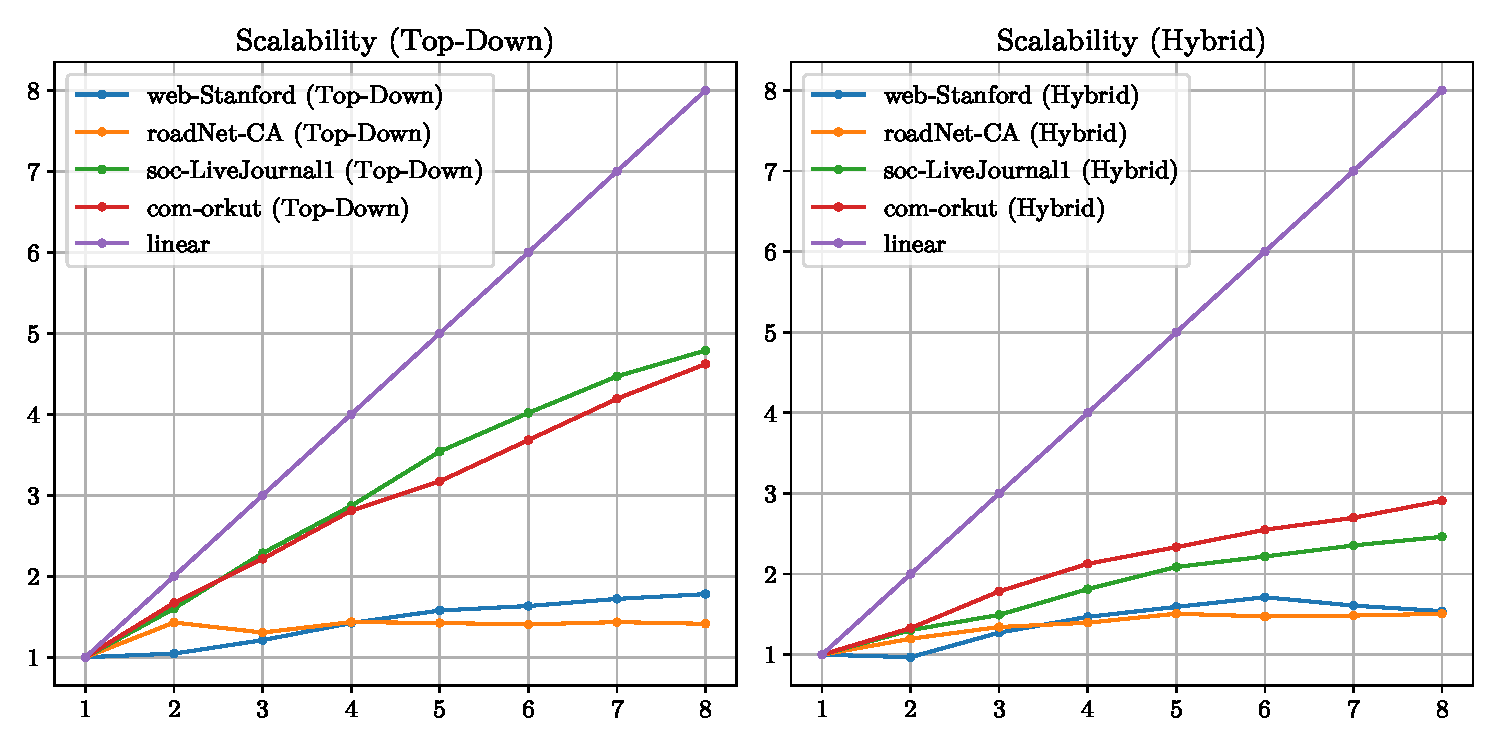
\includegraphics[width=\textwidth]{figures/scalability.pdf}
	\caption{Scalability}
\end{figure}

From \textbf{Figure 1.}, we can observe that generally, Top-Down method have better scalability than Hybrid method {\color{MaterialBlueGrey}\textbf{(TODO: check the experiments result)}}. We can have another table here \textbf{Table 2.},

\begin{table}[!ht]
	\centering
	\begin{tabular}{ c | c | c | c }
		\textbf{Case Name}          & \textbf{MTEPS (1)} & \textbf{MTEPS (8)} & \textbf{Speedup} \\
		\hline \hline
		web-Stanford (Top-Down)     & 449.4192           & 799.5279           & 1.7790           \\
		roadNet-CA (Top-Down)       & 74.1208            & 104.6878           & 1.4124           \\
		soc-LiveJournal1 (Top-Down) & 116.5680           & 558.0582           & 4.7874           \\
		com-orkut (Top-Down)        & 262.9554           & 1214.7666          & \textbf{4.6197}  \\
		\hline
		web-Stanford (Hybrid)       & 259.8544           & 400.0949           & 1.5397           \\
		roadNet-CA (Hybrid)         & 70.4230            & 106.1609           & 1.5075           \\
		soc-LiveJournal1 (Hybrid)   & 377.2501           & 928.8944           & 2.4623           \\
		com-orkut (Hybrid)          & 1463.4845          & 4257.6597          & 2.9093           \\
	\end{tabular}
	\caption{Speedup}
\end{table}

This graph reveals that, even though the scalability of Hybrid method is lower, the performance is significantly better.

\printbibliography

\end{document}
